\documentclass[12pt]{article}

% Solutions toggle
\newif\ifsolutions
\solutionsfalse
%% \solutionstrue

% ASSIGNMENT NUMBER
\newcommand{\hwnumber}{3}
\newcommand{\booksection}{}
\newcommand{\duedate}{}
% -------------

%%% Packages
\usepackage[margin=1in, footskip=24pt, headheight=24pt]{geometry}
\usepackage{amsmath, amssymb, amsthm, graphicx}
\usepackage{mathtools}
\DeclarePairedDelimiter\ceil{\lceil}{\rceil}
\DeclarePairedDelimiter\floor{\lfloor}{\rfloor}
\usepackage[colorlinks, urlcolor=blue]{hyperref}
\usepackage{color}
\usepackage{comment}
\usepackage{enumerate}
\usepackage{lastpage}
\usepackage{multirow, multicol}
\usepackage{tikz}
\usetikzlibrary{matrix,decorations.text,decorations.pathmorphing,decorations.markings,arrows,calc,shapes.geometric,patterns,shadows,intersections,decorations.markings,decorations.pathreplacing,decorations.pathreplacing,backgrounds,angles,quotes}
\usepackage{pgfplots}
\pgfplotsset{compat=1.16}

\usepackage{fancyhdr}

\pagestyle{fancy}
%% \renewcommand{\familydefault}{\sfdefault}

\newcommand{\R}{\mathbb{R}}
\newcommand{\ddx}{\frac{d}{dx}}

\global\long\def\V#1{\boldsymbol{#1}} %vector
\global\long\def\M#1{\boldsymbol{#1}} %matrix

\global\long\def\D#1{\Delta#1} %\D{t} for time step size
\global\long\def\d#1{\delta#1} %\d{t} for small increment

\global\long\def\norm#1{\left\Vert #1\right\Vert }
\global\long\def\abs#1{\left|#1\right|}

\global\long\def\grad{\M{\nabla}}
\global\long\def\av#1{\left\langle #1\right\rangle }

% HEADER MACROS
\newcommand{\term}{Spring 2022 \& 2023}
\newcommand{\coursename}{Intro Math Modeling}
\newcommand{\coursenumber}{MATH-UA 251}
\newcommand{\course}{\coursename \ (\coursenumber)}

\fancyhead[RO]{\term}
\fancyhead[LO]{\course}
% -------------

%%% Theorem Styles
\theoremstyle{definition}
\newtheorem{ex}{Exercise}

%%%%%%%%%%%%%%%%%%%%%%%% Solutions %%%%%%%%%%%%%%%%%%%%%%%%%%%%%
% \begin{solution} and \begin{answerspace} must be at the beginning of the line.
% Doesn't work inside the \myversions command. Use if statements instead.
% No underscores in comment names

\ifsolutions
\newenvironment{solution}{\color{blue}}{} \excludecomment{answerspace} \newenvironment{notes}{\color{red} \noindent Grading Notes:}{}
\else
\excludecomment{notes} \excludecomment{solution} \includecomment{answerspace} 
\fi
%%%%%%%%%%%%%%%%%%%% End Solutions %%%%%%%%%%%%%%%%%%%%%%%e}


\begin{document}
% HEADER
\begin{center}
%% \ifsolutions
%%   \textbf{\Large Homework \hwnumber\ - \booksection\ (Solutions)}\\
%% \else
%%   \textbf{\Large Homework \hwnumber\ - \booksection}\\
%% \fi
\ifsolutions
  \textbf{\Large Homework \hwnumber\ (Solutions)}\\
\else
  \textbf{\Large Homework \hwnumber}\\
\fi
\vspace{12pt}
Due date: someday, sometime! \duedate

Submit on NYU Brightspace.
\end{center}

%% \noindent Please give complete, well-written solutions to the following exercise. Provide sufficient justification and explanation for a classmate who has not worked on the exercise to understand your solution.


\begin{ex}
  
  [50 pts] Consider a straight rectangular heat fin illustrated below. Assuming steady-state conditions, write a thermal energy balance for the elemental volume of width $\Delta x$ (from $x$ to $x+\Delta x$) demarcated by the red solid lines. Then, let $\Delta x\to 0$ to find the governing ordinary differential equation.

  \begin{center}
    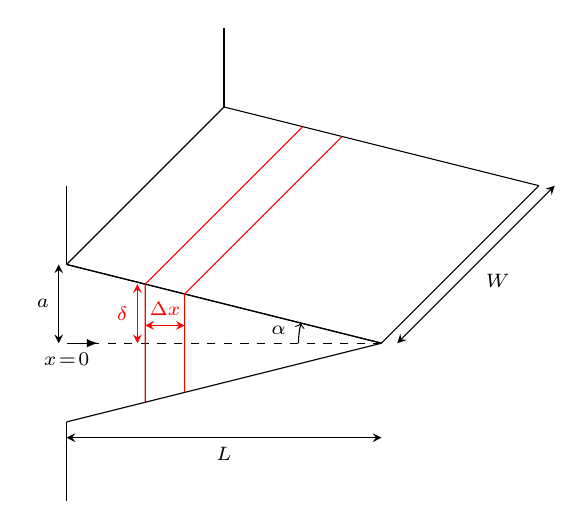
\begin{tikzpicture}
      \def\L{4}
      \def\a{1}
      \def\h{1}
      \def\wx{2}
      \def\wy{2}
      \coordinate (O) at (0,0);
      \coordinate (T) at (\L,0);
      \draw[dashed] (T) -- (O) coordinate (center);
      \draw (T) -- ($(O)+(0,\a)$) coordinate (upper);
      \draw (T) -- ($(O)+(0,\a)$) coordinate (upper);
      \draw ($(O)+(0,-\a)$) -- (T);
      \draw ($(O)+(0,\a)$) -- ($(O)+(0,\a)+(0,\h)$);
      \draw ($(O)+(0,-\a)$) -- ($(O)+(0,-\a)+(0,-\h)$);
      \draw ($(O)+(0,\a)+(\wx,\wy)$) -- ($(T)+(\wx,\wy)$);
      \draw (T) -- ($(T)+(\wx,\wy)$);
      \draw ($(O)+(0,\a)$) -- ($(O)+(0,\a)+(\wx,\wy)$);
      \draw ($(O)+(0,\a)+(\wx,\wy)$) --++ (0,\h);
      \def\al{0.4}
      \draw[->,>=latex] (O) --++ (\al,0);
      \node[anchor=north] at (O) {\scriptsize{$x\!=\!0$}};
      \draw[<->,>=stealth] ($(O)+(0,-1.2*\a)$) --++ (\L,0);
      \node[anchor=north] at ($(O)+(0,-1.2*\a)+(0.5*\L,0)$) {\scriptsize{$L$}};
      \draw[<->,>=stealth] ($(T)+(0.2*\a,0)$) --++ (\wx,\wy);
      \node[anchor=north west] at ($(T)+(0.2*\a,0)+(0.5*\wx,0.5*\wy)$) {\scriptsize{$W$}};
      \draw[<->,>=stealth] ($(O)+(-0.1*\a,0)$) --++ (0,\a);
      \node[anchor=east] at ($(O)+(-0.1*\a,0.5*\a)$) {\scriptsize{$a$}};
      
      \def\l{1}
      \def\dl{0.5}
      \pgfmathsetmacro\t{\a-\l*\a/\L}
      \draw[color=red] ($(O)+(\l,0)+(0,-\t)$) --++ (0,2*\t) --++ (\wx,\wy);
      \draw[<->,>=stealth,color=red] ($(O)+(\l,0)+(0,0.3*\t)$) --++ (\dl,0);
      \node[red,anchor=south] at ($(O)+(\l,0)+(0,0.3*\t)+(0.5*\dl,0)$) {\scriptsize{$\Delta x$}};
      \draw[<->,>=stealth,color=red] ($(O)+(\l-0.1*\a,0)$) --++ (0,\t);
      \node[red,anchor=east] at ($(O)+(\l-0.1*\a,0)+(0,0.5*\t)$) {\scriptsize{$\delta$}};
      \pgfmathsetmacro\t{\a-(\l+\dl)*\a/\L}
      \draw[color=red] ($(O)+(\l+\dl,0)+(0,-\t)$) --++ (0,2*\t) --++ (\wx,\wy);
      
      \pic [draw, <-, "{\scriptsize{$\alpha$}}", angle eccentricity=1.25, angle radius=30] {angle = upper--T--center};
      
    \end{tikzpicture}
  \end{center}
  
  You need to account for the unidirectional heat conduction within the fin, with flux $q_x=-kdT/dx$, and convection to the ambient, with flux $h(T-T_{\infty})$. The sides of the fin (the two triangles with base $2a$ and height $L$) are insulated, and thus, does not contribute to the convection to ambient. Here, the symbols stand for thermal conductivity, $k$ (assume constant); temperature of the fin, $T$; ambient temperature, $T_{\infty}$; horizontal distance from the base, $x$; and the convective heat transfer coefficient, $h$.
  
Next, change variable $y=2\sqrt{\gamma(L-x)}$ where $\gamma=hL/(ak\cos(\alpha))$, and $\theta=T-T_{\infty}$, and write the governing equation in terms of $y$ and $\theta$. You will reach to the modified Bessel equation of order zero, which should look like
  $$y^2\frac{d^2\theta}{{dy}^2}+y\frac{d\theta}{dy}-y^2\theta=0.$$
General solution to the above Bessel equation is
  $$\theta=C_1I_0(y)+C_2K_0(y),$$
  where $I_0(y)$ and $K_0(y)$ are the modified Bessel functions of the first and second kinds. For the boundary conditions, let $T=T_0$ at the base ($x=0$) and enforce a finite temperature at $x=L$. Find the coefficients $C_1$ and $C_2$, and express the final answer for $\theta$ in terms of $x$ and Bessel functions. \textbf{Hint: } $K_0(y)$ blows up ($\to\infty$) at $y=0$. 
  
\begin{solution}
  The balance equation can be expressed as
  $$\left(q_xA\right)_x-\left(q_xA\right)_{x+\Delta x}-hS(T-T_{\infty})=0,$$
  where $A(x)=2\delta W$ (with $\delta=a(1-x/L)$) and $S=2W\Delta x/\cos(\alpha)$ are the conduction and convection area, respectively. Substitute for the area and $q_x$, divide by $\Delta x$, and let $\Delta x\to 0$:
  \begin{align*}
    &\left(-k\frac{dT}{dx}(2\delta W)\right)_x-\left(-k\frac{dT}{dx}(2\delta W)\right)_{x+\Delta x}-\frac{2hW\Delta x}{\cos(\alpha)}(T-T_{\infty})=0,\\
    \Rightarrow&\lim_{\Delta x\to 0}\frac{\left(-k\frac{dT}{dx}(2\delta W)\right)_x-\left(-k\frac{dT}{dx}(2\delta W)\right)_{x+\Delta x}}{\Delta x}-\frac{2hW}{\cos(\alpha)}(T-T_{\infty})=0,\\
    \Rightarrow&\lim_{\Delta x\to 0}\frac{\left(-\delta\frac{dT}{dx}\right)_x-\left(-\delta\frac{dT}{dx}\right)_{x+\Delta x}}{\Delta x}-\frac{h}{k\cos(\alpha)}(T-T_{\infty})=0,\\
    \Rightarrow&-\frac{d}{dx}\left(-\delta \frac{dT}{dx}\right)-\frac{h}{k\cos(\alpha)}(T-T_{\infty})=0,\\
    \Rightarrow&\frac{d}{dx}\left(a\left(1-\frac{x}{L}\right)\frac{dT}{dx}\right)-\frac{h}{k\cos(\alpha)}(T-T_{\infty})=0.
  \end{align*}
  One can further simplify the final equation, the governing ODE, as
  \textcolor{teal}{$$(L-x)\frac{d^2T}{{dx}^2}-\frac{dT}{dx}-\gamma(T-T_{\infty})=0.$$
    with $\displaystyle{\gamma=\frac{hL}{ak\cos(\alpha)}}$.}

  Next, we let $y=2\sqrt{\gamma(L-x)}$ and $\theta=T-T_{\infty}$:
  \begin{align*}
    \frac{dT}{dx}=&\frac{dT}{dy}\frac{dy}{dx}=-\sqrt{\gamma}(L-x)^{-\tfrac{1}{2}}\frac{dT}{dy},\\
    \frac{d^2T}{{dx}^2}=&\frac{d}{dx}\left(-\sqrt{\gamma}(L-x)^{-\tfrac{1}{2}}\frac{dT}{dy}\right)=-\tfrac{1}{2}\sqrt{\gamma}(L-x)^{-\tfrac{3}{2}}\frac{dT}{dy}+\frac{\gamma}{L-x}\frac{d^2T}{{dy}^2}.
  \end{align*}
  Note that $\theta$ and $T$ differ by only a constant, and their derivatives are the same. Substituting the new derivative formula above into the governing equation yields
  \begin{align*}
    &(L-x)\left[-\tfrac{1}{2}\sqrt{\gamma}(L-x)^{-\tfrac{3}{2}}\frac{d\theta}{dy}+\frac{\gamma}{L-x}\frac{d^2\theta}{{dy}^2}\right]+\sqrt{\gamma}(L-x)^{-\tfrac{1}{2}}\frac{d\theta}{dy}-\gamma\theta=0,\\
    \Rightarrow&\gamma\frac{d^2\theta}{{dy}^2}+\frac{\sqrt{\gamma}}{2\sqrt{L-x}}\frac{d\theta}{dy}-\gamma\theta=0\Rightarrow\gamma\frac{d^2\theta}{{dy}^2}+\frac{\gamma}{y}\frac{d\theta}{dy}-\gamma\theta=0. 
  \end{align*}
  Finally, multiplying all terms by $y^2/\gamma$ gives\textcolor{teal}{$$y^2\frac{d^2\theta}{{dy}^2}+y\frac{d\theta}{dy}-y^2\theta=0,$$}%
  which is the modified Bessel equation of order zero with general solution
  $$\theta=C_1I_0(y)+C_2K_0(y)=C_1I_0(2\sqrt{\gamma(L-x)})+C_2K_0(2\sqrt{\gamma(L-x)}).$$
  Temperature should be finite at the tip of the fin, $x=L$, i.e., $C_1I_0(0)+C_2K_0(0)$ should be finite, which indicates that $C_2=0$ ($K_0(y)$ blows up and goes to $\infty$ at $y=0$). The other boundary condition is $\theta=\theta_0=T_0-T_{\infty}$ at $x=0$: $\theta_0=C_1I_0(2\sqrt{\gamma L})\Rightarrow C_1=\theta_0/I_0(2\sqrt{\gamma L})$. Therefore, the solution becomes\textcolor{teal}{$$\theta=\theta_0\frac{I_0(2\sqrt{\gamma(L-x)})}{I_0(2\sqrt{\gamma L})}.$$}%
\end{solution}
\end{ex}

\begin{ex}

  [50 pts] Consider a heated sphere of radius $R$, with constant surface temperature $T_R$, suspended in a large, motionless (no velocity), body of fluid at $T=T_{\infty}$. Assuming steady state conditions, find the temperature distribution within the fluid as a function of $r$, distance from the center of the sphere. Start by writing a heat energy balance for a spherical shell between $r$ and $r+\Delta r$ for an arbitrary $r>R$. Let $\Delta r\to 0$ and find the governing differential equation. Use the boundary conditions $T(R)=T_R$ and $T\to T_{\infty}$ as $r\to\infty$ to find the constants, and subsequently, the temperature distribution.

  Next, equate the conduction heat flux at the surface of the sphere to the total heat transfer to the ambient:
  $$\left(-k\frac{dT}{dr}\right)_{r=R}=h(T_{R}-T_{\infty}).$$
  Having the temperature distribution $T(r)$, solve the above equation for $h$, the heat transfer coefficient. Then show that the dimensionless heat transfer coefficient, known as the Nusselt number, $\mathrm{Nu}$, is
  $$\mathrm{Nu}=\frac{hD}{k}=2,$$
  in which $D$ is the sphere diameter.
\end{ex}

\begin{solution}
  We have
  $$\left(q_r 4\pi r^2\right)_r-\left(q_r 4\pi r^2\right)_{r+\Delta r}=0\Rightarrow\frac{d}{dr}\left(4\pi kr^2\frac{dT}{dr}\right)=0\Rightarrow r^2\frac{dT}{dr}=C_1\Rightarrow T=-\frac{C_1}{r}+C_2.$$
  Use $r\to\infty\Rightarrow T\to T_{\infty}$ to find $C_2=T_{\infty}$. At $r=R$: $T(R)=-C_1/R+T_{\infty}=T_R\Rightarrow C_1=R(T_{\infty}-T_R)$. Therefore, the temperature distribution is\textcolor{teal}{
    $$T=(T_R-T_{\infty})\frac{R}{r}+T_{\infty}.$$}%

  The flux balance on the surface is
  $$\left(-k\frac{dT}{dr}\right)_{r=R}=-k\left(-(T_R-T_{\infty})\frac{R}{r^2}\right)_{r=R}=\frac{k(T_R-T_{\infty})}{R}=h(T_R-T_{\infty}).$$
  Therefore, $h=k/R$, and\textcolor{teal}{
  $$\mathrm{Nu}=\frac{h(2R)}{k}=2.$$}
\end{solution}
\end{document}
